\chapter{Optomechanical topology optimization problems}\label{chap:om}
%\section{Opto-mechanical systems~\cite{ownpub1,ownpub2,ownpub3}}\label{sec:optomechanics}
Optomechanics, the study of the interaction between light and mechanical motion, is at the heart of state-of-the-art technologies, such as 
optical trapping~\cite{ashkin_acceleration_1970, moffitt_recent_2008} and cooling~\cite{cooling}, quantum information processing~\cite{Andrews_2014, Xi_2025}
, light sails~\cite{lightsail, lightsail1}, and high-precision metrology and sensing~\cite{sensing, weakforce, Li:18, Mason_2019}. The most basic description of this interaction is given by the \textbf{Lorentz force}, which governs how moving charges respond to electric and magnetic fields
\begin{equation}\label{eq:lorentz_f}
 \mathbf{\bm{\mathcal{F}}}(\mathbf{r},t) = q \left[ \bm{\mathcal{E}}(\mathbf{r},t) + \mathbf{v}(t) \times \bm{\mathcal{B}}(\mathbf{r},t) \right]\,,
\end{equation}
where $q$ is the charge and $\mathbf{v}$ is the velocity of the particle. This force can be generalized to describe more complex systems,
such as the force between two current-carrying 
wires (Ampère's force law), and the electromotive force, which is at the core of many technologies, such as induction motors or generators.
In optomechanical systems, shaping the distribution and magnitude of these forces at the micro- and nanoscale is crucial for controlling mechanical motion with light. 
However, designing structures that can efficiently harness and manipulate these interactions often requires navigating highly complex
 parameter spaces and trade-offs between optical, mechanical, and material constraints.

 Topology optimization is one effective approach for enhancing and shaping optomechanical interactions.
Recent advances in optomechanical topology optimization include the design of devices harnessing the coupling between optical and elastic
 waves~\cite{photo_topopt}, optical systems with nonlinear deformations~\cite{def_wg}, high-$Q$ optomechanical membranes~\cite{highQ1, fengwen, aragon1},
light sail structures~\cite{lightsail_topopt, lightsail_topopt1},
photonic~\cite{ownpub1} and plasmonic~\cite{nelson_inverse_2024} particle trapping devices, optical force-based particle manipulation~\cite{ownpub2, particle_opt},
and structural integrity constraint formulations~\cite{structural_integrity},
 among others.

 In the following sections, we highlight our contributions to the field by solving topology optimization problems in three distinct regimes: a general treatment based on the Maxwell stress tensor~\cite{ownpub2}, 
 the dipole approximation in the small particle limit~\cite{ownpub1, ownpub3}, and strongly coupled systems where optical forces can induce significant mechanical deformations.
\section{The Maxwell stress tensor formalism~\cite{ownpub2}}\label{sec:engi}

In the most general case, the optical force can be calculated using the \textbf{Maxwell stress tensor} (MST) formalism, which is a generalization of the Lorentz force (\eqref{eq:lorentz_f}) in continuous media~\cite{novotny}.
The basic idea is sketched in \figref{fig:eng_res}~(a), where
a particle scatters an incident time-harmonic electromagnetic field $\mathbf{E}_\text{inc}$, creating the time-harmonic scattered field $\mathbf{E}_\text{scat}$ and the net force $\mathbf{F}$ that acts
on the particle. The net time-averaged force is given by~\cite{novotny}
\begin{equation}\label{eq:f_MST}
    \mathbf{F}(\mathbf{r}) \equiv \langle\bm{\mathcal{F}}(\mathbf{r}, t)\rangle=\int_{\Gamma}\langle\stackrel{\leftrightarrow}{\bm{\mathcal{T}}}(\mathbf{r}, t)\rangle \cdot \mathbf{n}_{\Gamma}(\mathbf{r}) \d \Gamma\,,
\end{equation}
where $\Gamma$ denotes any boundary enclosing the particle, $\mathbf{n}_{\Gamma}$ denotes the unitary vector normal to that boundary, $\bm{\mathcal{F}}$ denotes the time-dependent force, and
the time-average of the stress tensor is given by
\begin{equation}
        \langle \stackrel{\leftrightarrow}{\bm{\mathcal{T}}}(\mathbf{r}, t) \rangle 
        = \frac{1}{2} \Re \Big\{ 
            \varepsilon\, \mathbf{E}(\mathbf{r}) \otimes \mathbf{E}^*(\mathbf{r})
            + \mu\, \mathbf{H}(\mathbf{r}) \otimes \mathbf{H}^*(\mathbf{r})
         - \frac{1}{2} \big( \varepsilon\, |\mathbf{E}(\mathbf{r})|^2 + \mu\, |\mathbf{H}(\mathbf{r})|^2 \big) 
        \stackrel{\leftrightarrow}{\mathbf{I}} \Big\}\,,
\end{equation}
where $\otimes$ denotes the outer product. Note that the permittivity ($\varepsilon$) and permeability ($\mu$) correspond to those of the medium surrounding the particle.

\begin{figure}[tb]
    \centering
    \makebox[\textwidth][c]{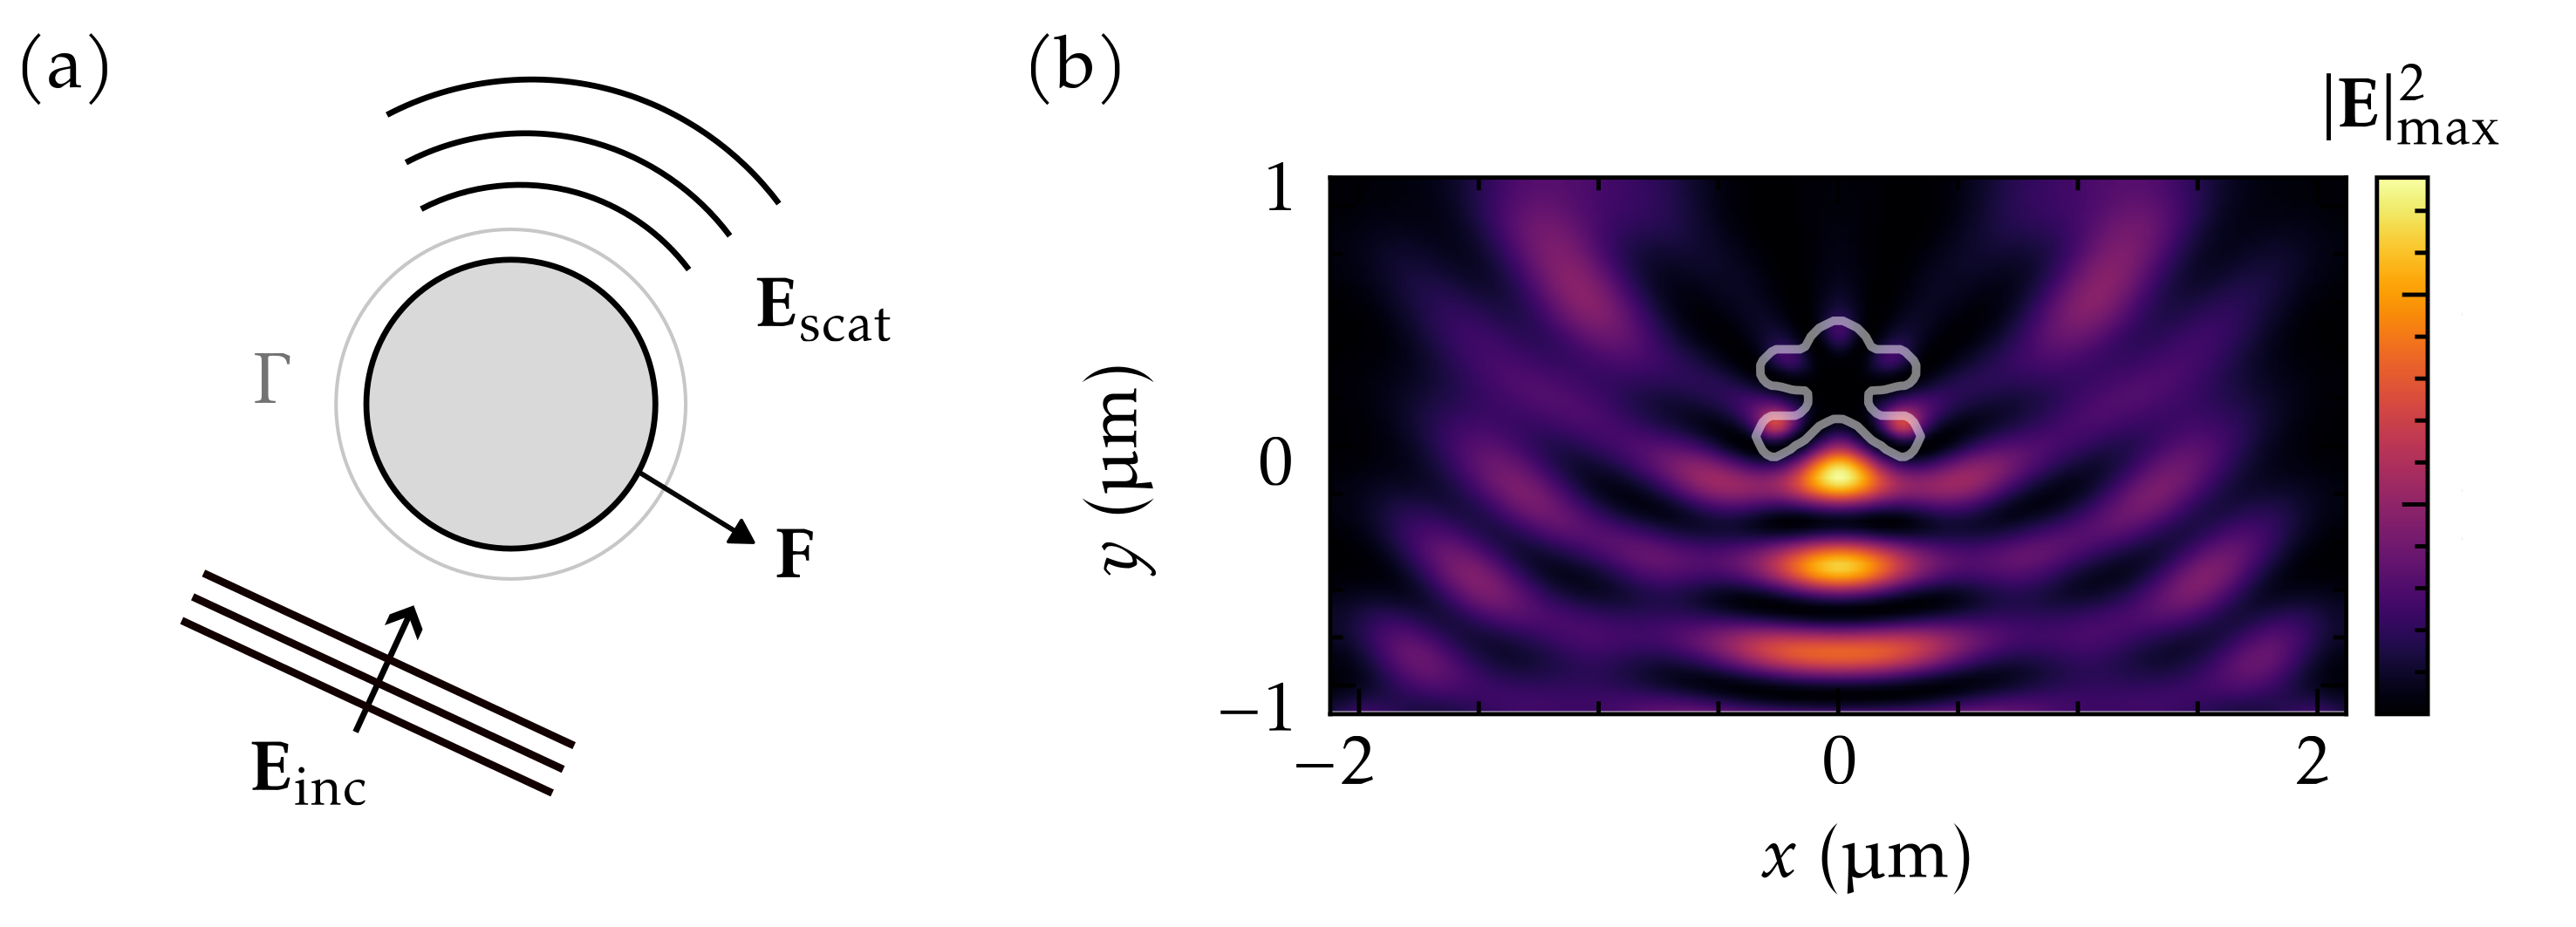
\includegraphics{figures/eng_results.png}}%%
    \caption{Topology optimization in optical force applications. (a) A scattering particle 
    enclosed by a boundary $\Gamma$ scatters a field $\mathbf{E}_\text{scat}$, when excited by an incident field $\mathbf{E}_\text{inc}$, 
    generating a net optical force $\mathbf{F}$. (b) Electric-field intensity distribution for a particle design optimized to maximize the vertical ($y$)
    component of the optical force. Figure adapted with permission from~\cite{ownpub2} © Optical Society of America.}
    \label{fig:eng_res}
\end{figure}

\subsection*{Engineering optical forces via topology optimization}

In~\cite{ownpub2} we apply this formalism to optimize two-dimensional particle--metalens geometries for different applications, such as attracting, repelling, 
oscillating, and trapping particles. In~\figref{fig:eng_res}~(b), we show an example optimization result from this work, where we optimize the geometry of a particle to maximize the vertical component of the optical force. 
The figure of merit is defined as $\text{FOM} = \mathbf{F} \cdot \mathbf{n}_y$, where $\mathbf{n}_y = (0, 1)$ is a unit vector in the vertical direction and 
the optical force $\mathbf{F}$ (\eqref{eq:f_MST}) is computed by integrating the Maxwell stress tensor around the design domain. 

The results in~\figref{fig:eng_res}~(b) show that the optimized particle geometry is a Bragg-mirror-like
structure, which can efficiently reflect the incoming plane wave, resulting in an efficient exchange of force and momentum. As a matter of fact, by comparing the response of the optimized design
to a reference square particle, we find that the topology-optimized device feels a $\approx 3\times$ stronger vertical force than the reference.
 Moreover, in~\cite{ownpub2} we show that by designing a metalens to focus the incoming plane wave onto the particle, one can utilize nearly all the momentum available in the simulation domain\footnote{This compares the calculated force with the radiation pressure force on a perfectly reflecting surface spanning the entire simulation domain~\cite{ownpub2}.},
 allowing for a $\approx 13\times$ stronger force than the reference square particle in free space. 
 In the remainder of~\cite{ownpub2} we further extend these examples by designing
attractive particle geometries, and optical-tweezer-like setups to trap the particle in space. All the code developed in this work is available on our GitHub~\cite{github_MST} repository, with tutorials on force calculation and topology optimization. 

One noteworthy aspect of the topology optimization of particles in the MST formalism is that, with our current framework, the particle cannot feature disconnected members; otherwise, instead of integrating around the whole design domain,
one would need to integrate around the (disconnected) individual components
 to calculate their individual force contribution (\eqref{eq:f_MST}). It is possible to solve this problem by enforcing 
a connectivity constraint via the VTM~\cite{li_structural_2016} (\secref{sec:aux}). In our examples,
we enforce particle connectivity to the center of the particle and connect the metalens structure to the bottom to ensure the structural
integrity of the structure.

\subsection*{Outlook and future work}

This topology optimization work is the first, to our knowledge, to 
target optical forces via the MST formalism, paving the way for future work in three-dimensional systems and more complex optimization problems, such as optically-driven particle
trajectory control~\cite{zemanek_perspective_2019, macdonald_microfluidic_2003, shilkin_directional_2017}, many-body particle systems~\cite{bechinger_active_2016, chang_colloquium_2018} or optically actuated devices~\cite{ivanyi_optically_2024}, among others. It is worth noting that an exciting and straightforward extension of the framework would be to use the MST formalism to calculate and optimize for the time-averaged torque acting on a particle, defined as~\cite{novotny}
\begin{equation}\label{eq:torque}
    \langle \bm{\tau} \rangle = \langle \mathbf{r} \times \bm{\mathcal{F}} \rangle = - \int_{\Gamma} \langle \stackrel{\leftrightarrow}{\bm{\mathcal{T}}}(\mathbf{r},t)
    \times \mathbf{r} \rangle \cdot \mathbf{n}_{\Gamma}(\mathbf{r}) \d\Gamma \,,
\end{equation}
where $\mathbf{r}$ is the vector defined between the rotation axis and the force application point. This definition of torque accounts
for two kinds of rotational motion; \textit{spinning} ($\langle \bm{\tau}_S \rangle$), where the particle rotates around its center of mass,
and \textit{orbiting} ($\langle \bm{\tau}_O \rangle$), where the particle rotates around an external axis, so that the total torque is the sum
of both the spin and orbital torque $\langle \bm{\tau} \rangle = \langle \bm{\tau}_S \rangle + \langle \bm{\tau}_O \rangle$~\cite{torque}.  Defining 
an optical torque-based FOM could open the door for the design of efficient optical and biological micro- and nanomachines~\cite{rotating, gluck}.

\section{The dipole approximation~\cite{ownpub1, ownpub3}}\label{sec:dip}

When particles are much smaller than the wavelength of the electromagnetic field 
($s \ll \lambda$), the optical force can be described using the dipole approximation 
in the quasistatic limit (\secref{sec:nanophotonics}). In this approximation, the 
particle is treated as a point dipole with a complex polarizability $\alpha$ that 
describes its response to the local electric field. 
The time-averaged optical force on the dipole is given by~\cite{novotny}
\begin{equation}\label{eq:dip_force}
    \mathbf{F} = 
    \underbrace{\frac{\alpha^{\prime}}{4} \nabla\left\{ \mathbf{E}^* \cdot \mathbf{E} \right\}}_{(\text{GF})}
    + \frac{\alpha^{\prime\prime}k}{\varepsilon_0}
    \Big[\, \underbrace{\frac{1}{c} \langle \mathbf{S} \rangle}_{(\text{RPF})}
    + \underbrace{c \big( \nabla \times \langle \mathbf{L} \rangle \big)}_{(\text{SCF})} \Big]\,,
\end{equation}
where the polarizability $\alpha = \alpha^\prime + i\,\alpha^{\prime\prime}$ is split into 
real and imaginary parts, $\langle \mathbf{S} \rangle = \frac{1}{2} \Re\{\mathbf{E} \times 
\mathbf{H}^*\}$ is the time-averaged Poynting vector, and 
$\langle \mathbf{L} \rangle = \frac{\varepsilon_0}{4 i \omega} (\mathbf{E} \times \mathbf{E}^*)$ 
is the time-averaged angular momentum. The real part of the polarizability ($\alpha^\prime$) produces the 
\textbf{gradient force} (GF), which is conservative and pulls the particle toward regions 
of varying field intensity. The imaginary part of the polarizability ($\alpha^{\prime\prime}$) 
gives rise to non-conservative scattering forces: the component associated with the Poynting vector is 
the radiation pressure force (RPF), which pushes the particle in the direction of energy 
flow, and the term associated with the angular momentum is the spin-curl force (SCF), 
which can induce transverse motion. 

In the abscence of absorption effects ($\alpha^{\prime \prime}=0$ and $\underbar{n}=n$ in \eqref{eq:perm}), the force is totally described 
by the conservative gradient force, which can be written as the gradient 
of a potential
\begin{equation}
    U (\mathbf{r}) = -\frac{\alpha^{\prime}}{4} \left|\mathbf{E}(\mathbf{r})\right|^2\,,
\end{equation}
where the force can be calculated as $\mathbf{F} = -\nabla U(\mathbf{r})$. In optical trapping applications, $U$ is often referred to as the \textbf{trapping potential}.
For non-resonant and non-absorbing isotropic particles, the polarizability is 
described through the relation~\cite{BornWolf:1999:Book} 
    $\alpha^{\prime}= 3 \varepsilon_0 V (\varepsilon_p-\varepsilon_m)/(\varepsilon_p+2 \varepsilon_m)\,,$
where $V$ is the volume of the particle, $\varepsilon_p$ and $\varepsilon_m$ are the relative
dielectric permittivities of the particle and the background medium, respectively. 

Note that in the dipole approximation for infinitesimally small particles, the field $\mathbf{E}$ is not modified by the presence of the particle.
This works well for point-like particles in free space but not necessarily 
for large particles, high refractive index contrasts between the particle and the background medium, or particles close to material
boundaries (e.g., optical cavities). The interaction between the background field and the particle can be accounted for in the dipole
approximation by considering the \textbf{self-induced back-action} (SIBA) effect, which assumes a weak
perturbation of the field due to the presence of the particle and expands the field in a perturbation series in terms of 
the scattering Green function of the particle~\cite{novotny, SIBA, benjamin}. If the series converges, the force calculated from the field 
using \eqref{eq:dip_force} should approach the result from the MST calculation in \eqref{eq:f_MST}. 
This agreement is often used to validate the dipole approximation (e.g., \cite{ownpub1,ownpub3}).

\subsection*{On-chip omnidirectional optical trapping via topology optimization~\cite{ownpub1}}

Based on the dipole approximation formalism, in ~\cite{ownpub1}, we demonstrate that topology optimization can be used to design an integrated \textbf{omnidirectional trapping} optical cavity, which was previously achievable only with free-space optical tweezers~\cite{ashkin_acceleration_1970} or bulky photonic devices~\cite{manka_simulation_2024}. The trapping device
consists of two silicon waveguides connected to a central design domain in which
topology optimization is applied [\figref{fig:MST_dipole} (a)]. The central region contains a cylindrical air exclusion with a radius
$R_\text{exc}=300$ nm and a thickness of $800$ nm, in which the stable trap is located.
To design an omnidirectional trapping device, we minimize  
the difference of the electric-field norm with respect to the electric-field norm of a reference field $\mathbf{E}_\text{ref}$
\begin{equation}
 \text{FOM} =\sqrt{\int_{\Omega}\left[\Theta_{\beta,\eta}\left(\frac{|\mathbf{E}(\mathbf{r})|}{\left|\mathbf{E}\left(\mathbf{r}_0\right)\right|}-\frac{\left|\mathbf{E}_{\text{ref}}(\mathbf{r})\right|}{\left|\mathbf{E}_{\text{ref}}\left(\mathbf{r}_0\right)\right|}\right)\right]^2 \text{~d} \Omega}\,,
    \end{equation}
where the fields are normalized with respect to the value at the center of the cavity ($\mathbf{r}_0$), and $\Theta_{\beta,\eta}$ is the smoothed Heaviside threshold (\eqref{eq:threshold}), which ensures
potentials as steep or steeper than the reference. The reference is chosen as a Gaussian trapping potential with standard deviations $\sigma_x=\sigma_y=300$ nm and $\sigma_z=400$ nm, but can be chosen to have any other form, such as a harmonic potential ($U\propto\mathbf{r}^2$).

\begin{figure}[tb]
    \centering
    \makebox[\textwidth][c]{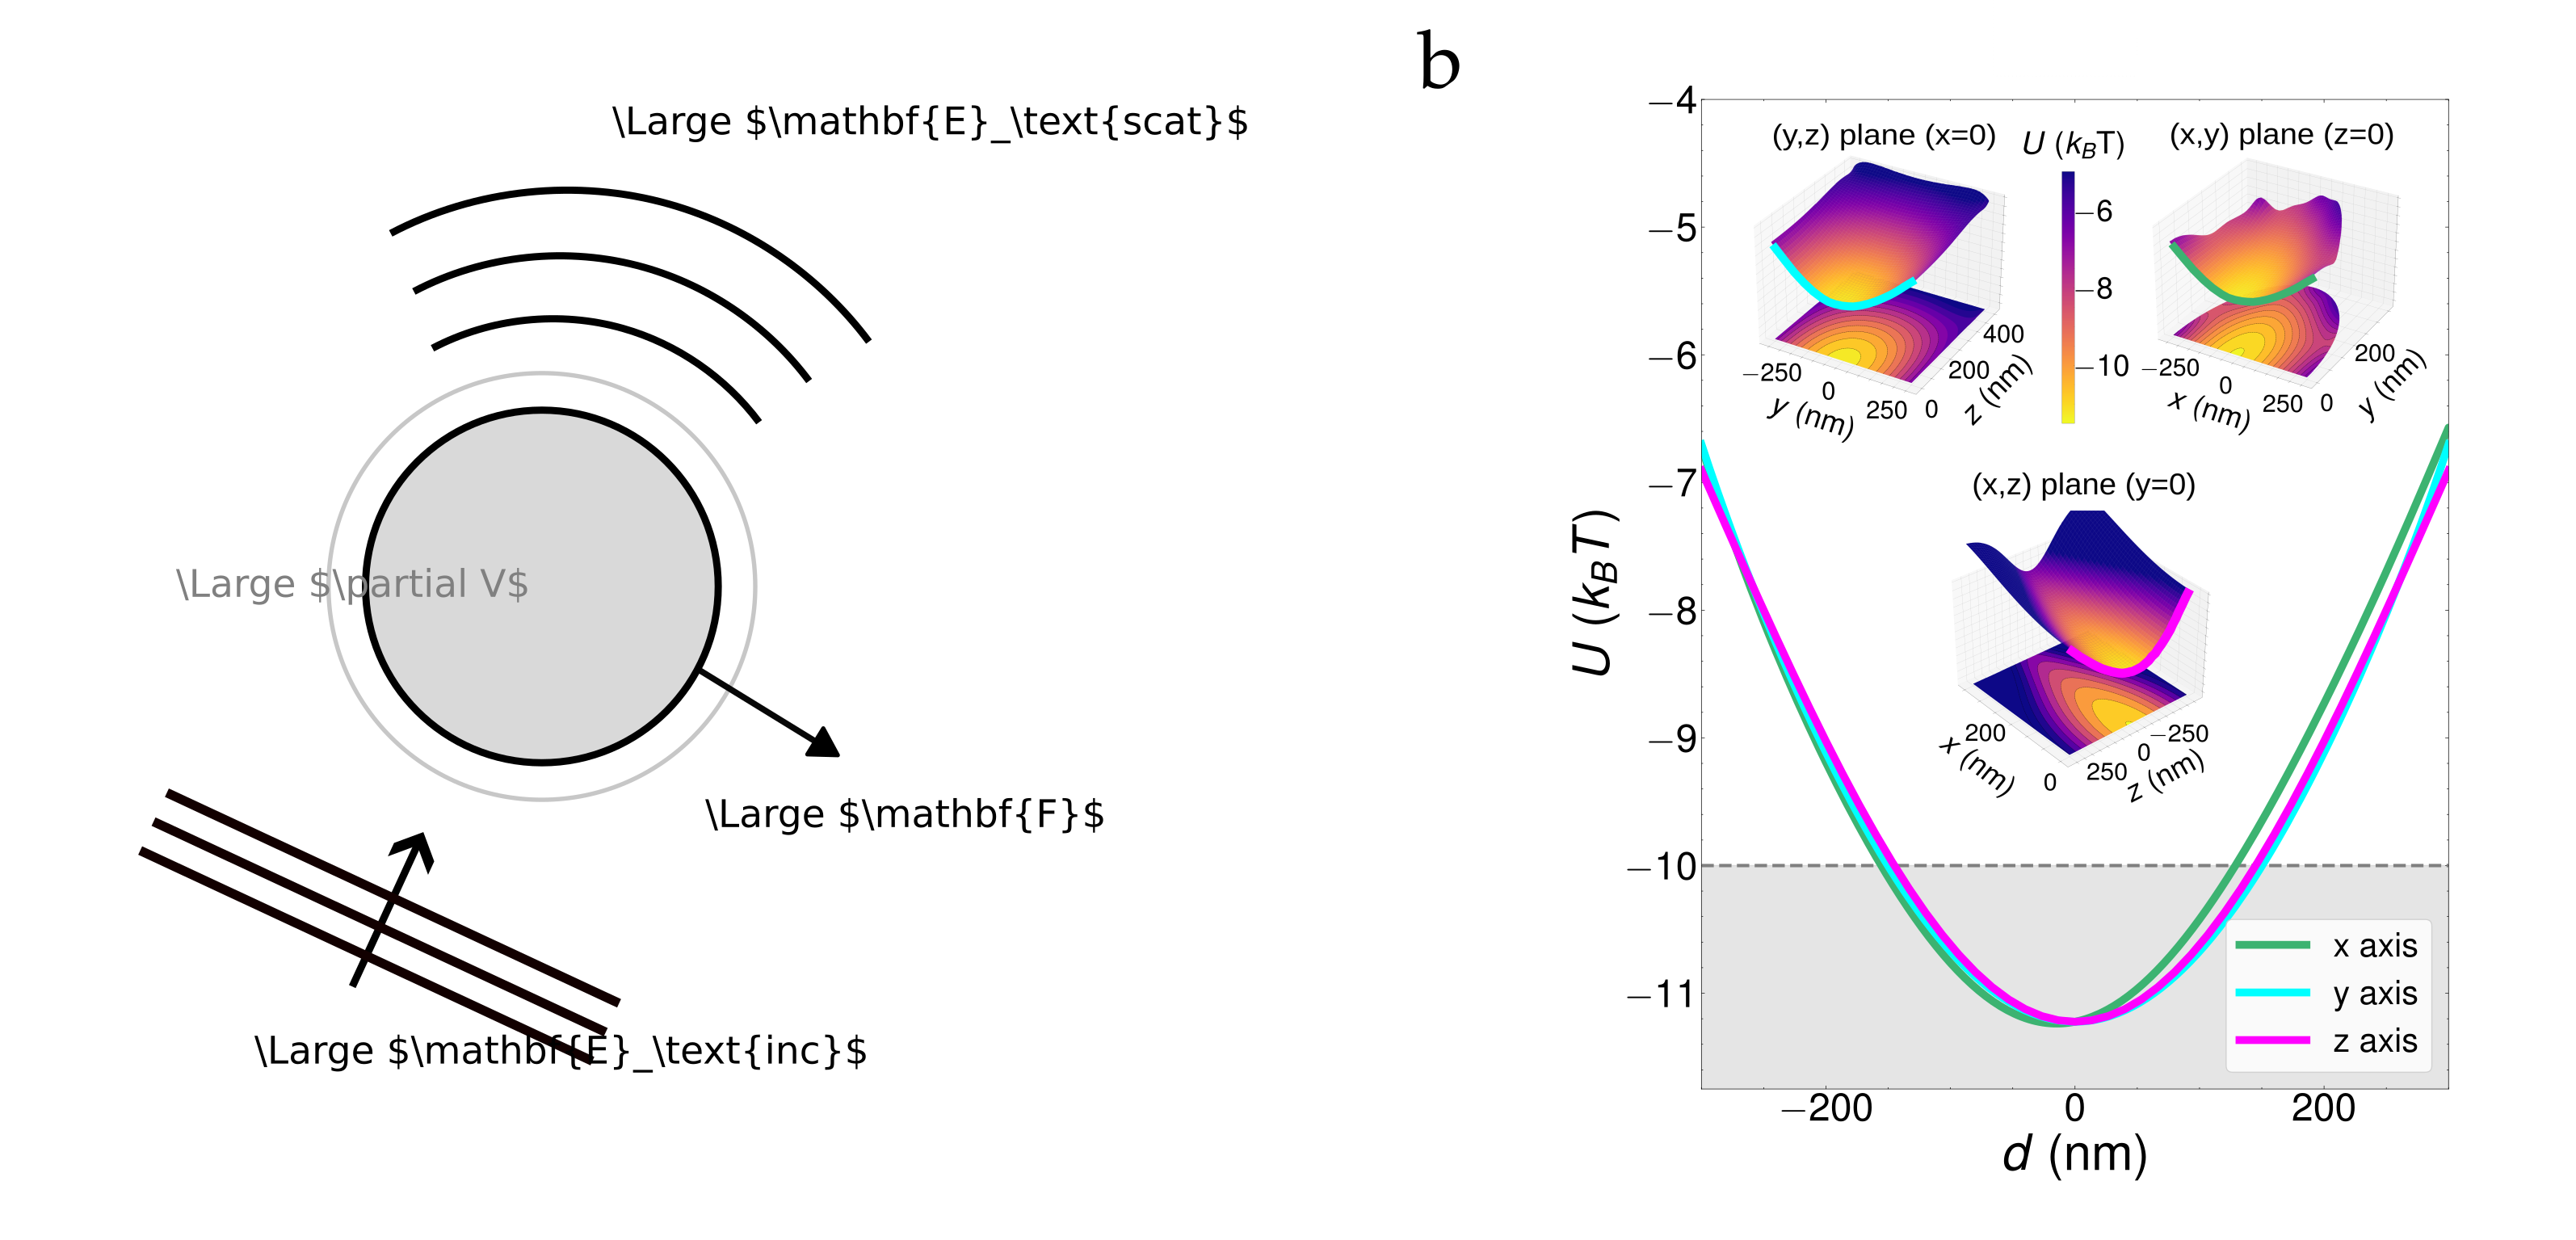
\includegraphics{figures/MST_dipole.png}}%%
    \caption{Optical response and trappig potential for the topology-optimized particle trap. (a) Lower half ($z<0$) of the optimized cavity, with the electric-field intensity
    distribution when excited with the fundamental waveguide mode with an input power of $P_\text{in}=60$ mW at $\lambda=1.55$ \textmu m. (b) Trapping potential for a $R=15$ nm and $n=2$ particle in the cavity region for the different axial line- and plane-cuts as a function
    of the distance from the center $d$, with the stable trapping regime ($U<-10 k_B\, T$) highlighted in gray. Figure adapted with permission from~\cite{ownpub1} © 2024 American Chemical Society.}
    \label{fig:MST_dipole}
\end{figure}

By applying this optimization framework, we obtain the topology-optimized cavity design in \figref{fig:MST_dipole} (a), which can trap particles at the center of an optical
cavity in three dimensions and has an associated Gaussian-like trapping potential [\figref{fig:MST_dipole} (b)], with a depth  $U<-10\, k_B T$\footnote{This depth is conventionally required to overcome Brownian fluctuations and ensure stable trapping~\cite{novotny}.}, where $k_B$ is the Boltzmann constant, for a deeply sub-wavelength particle with radius $R=15$ nm and refractive index $n=2$, at room temperature ($T=300$ K).
Since the framework is based on the dipole approximation,
as long as the approximation is valid, it allows to trap arbitrarily small particles by tuning the input power.

From the dipole approximation trapping potential, we calculate the force-displacement curves and we determine trapping stiffnesses
of $K \approx 0.5$ fN/nm, an order of magnitude larger than diffraction-limited free-space optical tweezers~\cite{ownpub1}. To validate these findings,
we employ the MST formalism (\secref{sec:engi}) to calculate the force on spherical particles as they are displaced from the cavity center and find excellent
agreement with the dipole approximation~\cite{ownpub1}. As shown in \figref{fig:SPIE}, to further verify the the dipole approximation assumption, in~\cite{ownpub3}, we compare the results of the dipole approximation with the MST
for varying spherical particle radii ($R_\text{sph}$) and refractive indices ($n_\text{sph}$), showing good agreement between the two methods
even for very large values of the refractive index (e.g., $n_\text{sph}=8$) and particle sizes up to $s \sim R_\text{sph}\approx 0.05 \lambda$, highlighting the versatility of the optimized device.

\subsection*{A metric for trapping performance~\cite{ownpub1}}

When designing optical trapping platforms, it is important to be able to compare performance across platforms. To this end, in~\cite{ownpub1}, we introduce a \textbf{normalized
trapping stiffness} metric, which normalizes trapping stiffness to input power ($P_\text{in}$) and particle  polarizability
\begin{equation}
 e_j=\frac{K_j \varepsilon_0}{\alpha^\prime P_{\text{in}}}\,,
\end{equation}
where $j \in \lbrace x,y,z \rbrace$ is an axis index. This metric enables one-to-one comparison across trapping devices\footnote{As noted in~\cite{ownpub1} this metric diverges for lightless platforms (e.g., Casimir force-based traps), where the metric could be redefined
without including the input power $e_j=K_j \varepsilon_0/\alpha^\prime$.}. The normalized trapping stiffness allows us to show that (Tab. 1 in~\cite{ownpub1}), although plasmonic devices can reach larger values of the normalized 
stiffness, they suffer from optical losses to heating and lack omnidirectional stable trapping. In contrast, the inverse-designed dielectric platform in \figref{fig:MST_dipole}
 achieves comparable normalized stiffnesses to other dielectric traps while uniquely offering fully stable, omnidirectional trapping
 without relying on SIBA effects. Notably, SIBA-based devices are particle-specific, and their functionality can break down
 for different particle geometries or materials. Compared to conventional optical tweezers, our device maintains similar trapping
 strength at lower input power due to its integrated, waveguide-coupled design, highlighting the benefits of miniaturized,
 near-field-based optical trapping.

 \begin{figure}[tb]
    \centering
    \makebox[\textwidth][c]{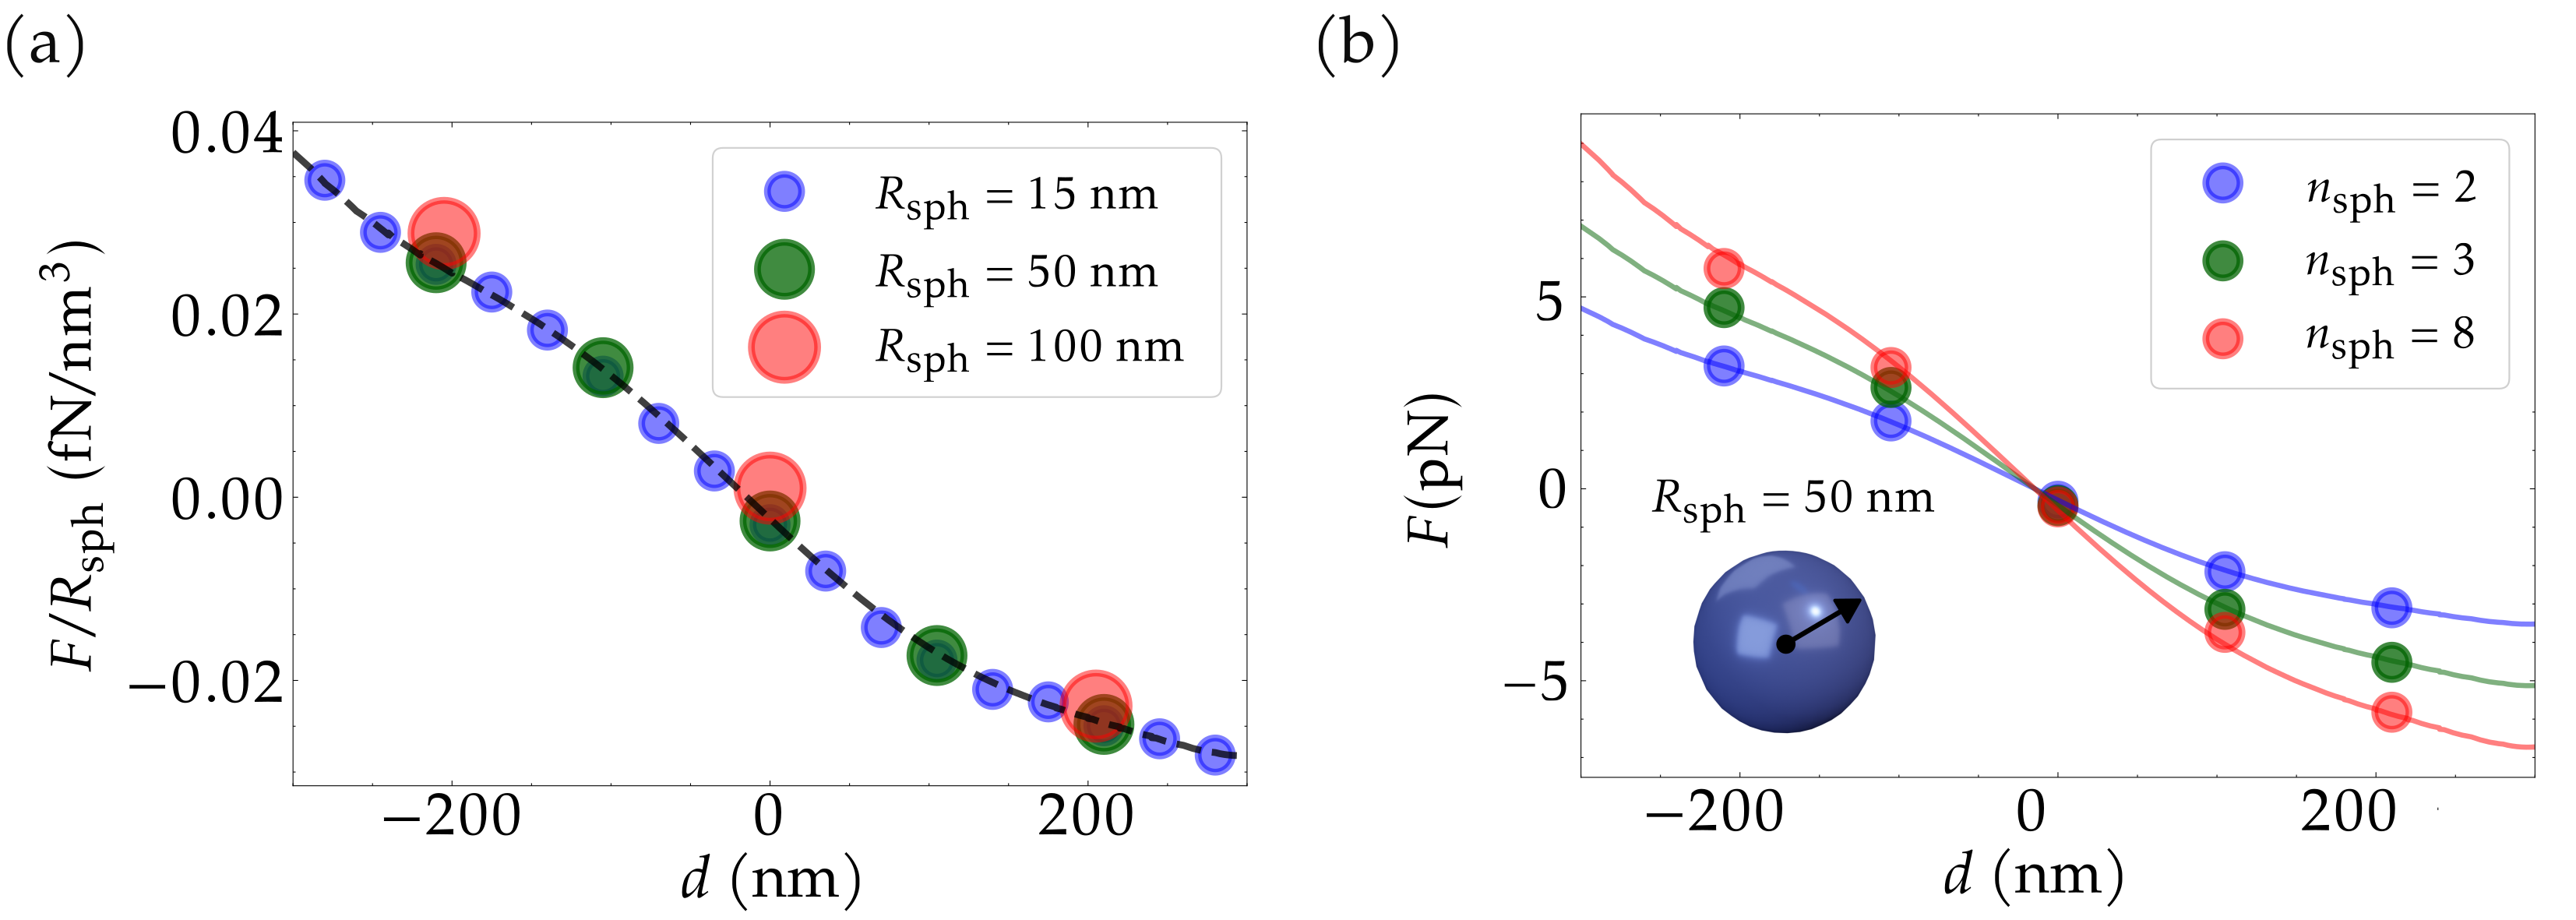
\includegraphics{figures/SPIE_results.png}}%%
    \caption{Validating the dipole approximation force calculation (dashed line) against the MST force calculation (data points), as a function of displacement ($d$) from the cavity center along the $x$-axis.
    (a) Volume-normalized force ($F/R^3_\text{sph}$) for different particle sizes with refractive index $n_\text{sph}=2$. (b) Force for different refractive indices of the particle for a particle radius $R_\text{sph}=50$ nm. Figure adapted with permission from~\cite{ownpub3} © 2024 IEEE.}
    \label{fig:SPIE}
\end{figure}

\subsection*{Outlook and future work}

Aside from the results presented here, in~\cite{ownpub1}, we discuss the influence of Casimir-Polder effects
 on particle loading and prospective applications of the proposed devices in optomechanics and biophotonics. The demonstrated on-chip, omnidirectional trapping enables strong confinement with low input power, offering a compact platform for manipulating deeply subwavelength particles and advancing both applied and fundamental research.

Future work could focus on extending the inverse design framework to support alternative materials, 
traps for lossy or resonant particles, and devices with multiple trapping sites.
 Such developments could enable scalable arrays of trapped quantum emitters, with potential applications
  in quantum optics and many-body physics~\cite{chang_colloquium_2018}. We anticipate that experimental demonstrations
   will validate these predictions and push the limits of integrated omnidirectional trapping.

\section{Strongly coupled optomechanical systems~\cite{ownpub5}}\label{sec:mech_strongly_coupled}

In strongly coupled optomechanical systems, the optical field can cause significant deformations of the device,
 which in turn can alter its optical response. In most optomechanical systems the optical response is much faster than the mechanical response, since the 
mechanical frequencies ($\omega_\text{mech}$) are orders of magnitude lower than the optical frequency ($\omega_\text{mech}\ll\omega$) or optical resonance decay rates ($\omega_\text{mech}\ll\gamma$, so one 
can neglect sideband cooling or amplification)~\cite{opto_crys, photo_topopt, ownpub5}. Due to the slower mechanical dynamics, it is possible to analyze the mechanical response of the structure in the quasistatic approximation, by only considering the mechanical steady-state response. 
This can be accounted for by considering the time-averaged MST force (\eqref{eq:f_MST}) in the continuum mechanics momentum equation
\begin{equation}\label{eq:mech}
    \nabla \cdot \overleftrightarrow{\boldsymbol{\sigma}} = \mathbf{f}_\text{MST}  \,,
\end{equation}
where the volumetric force density from the MST is given by $ \mathbf{f}_\text{MST} = \nabla \cdot \langle \stackrel{\leftrightarrow}{\bm{\mathcal{T}}} \rangle$ (\eqref{eq:f_MST}) and $\overleftrightarrow{\boldsymbol{\sigma}}$ is the stress tensor of the mechanical system. Solving the mechanical problem for the
displacement field $\mathbf{u}$ [e.g., via the finite element method (\secref{sec:fem})~\cite{cook_concepts_2001}], one can find the deformed configuration of a structure. Together, the 
solutions to the mechanical problem (\eqref{eq:mech}) and the optical problem (\eqref{eq:wave_eq}) 
form the foundation for addressing strongly coupled optomechanical systems. Another possibility of including further optomechanical coupling would be to consider
photoelastic effects, where the in-material strain modifies the material refractive index~\cite{photoelasticity}.

\subsection*{Topology optimization of strongly coupled optomechanical membranes}

To illustrate the use of topology optimization for strongly coupled optomechanical problems, we consider the two-dimensional model of an optomechanical membrane-like device presented in~\cite{ownpub5}. 
This system consists of a clamped-clamped membrane connected to a central design domain (Fig. 1 in~\cite{ownpub5}). The device is excited by an incoming plane wave from the bottom of the simulation domain, which generates a mechanical volumetric load on the structure,
resulting in an upwards deformation of the membrane. The goal of the optimization problem is to target the system's optomechanical coupling by maximizing the vertical component of the displacement ($u_y$) at a point ($\mathbf{r}_0$)
in the structure, such that $\text{FOM}=u_y(\mathbf{r}_0)$.

We solve the strongly coupled optomechanical problem by considering an optical frequency-domain problem (\eqref{eq:wave_eq}) coupled to a geometrically nonlinear mechanical problem~\cite{ownpub5,cook_concepts_2001}. Discretizing the system via the finite element
method (\secref{sec:fem}) yields the coupled system of equations
\begin{equation}\label{eq:coupled}
    \begin{aligned}
 \mathbf{K}\left(\alpha\mathbf{U}\right) \mathbf{E} &= \mathbf{E}_\text{in} , \\
 \mathbf{R}[\mathbf{U}, \mathbf{F}_\text{MST}(\mathbf{E})] &=\mathbf{0}\,,
    \end{aligned}
    \end{equation}
where $\mathbf{K}$ is the discretized system matrix which encodes the operators
 in the linear optical problem, $\mathbf{E}$ and 
 $\mathbf{E}_\text{in}$ are the vectors containing the nodal degrees-of-freedom for the electric 
field and the forcing term, respectively, $\mathbf{R}$ is the residual of the
 geometrically nonlinear mechanical problem~\cite{cook_concepts_2001}, and 
 $\mathbf{U}$ and $\mathbf{F}_\text{MST}$ are the vectors containing the nodal
 degrees-of-freedom for the displacement field and the time-averaged MST forcing term, respectively. 
 Moreover, we consider the parameter $\alpha$, which allows us to control if we solve 
 the strongly coupled problem ($\alpha=1$), where the optical field deforms the structure, 
 or the weakly coupled problem ($\alpha=0$), which is a good approximation in the small deformation 
 limit ($\alpha\mathbf{U} \ll 1$). To solve the strongly coupled problem in 
  \eqref{eq:coupled} we use a segregated scheme (\secref{sec:coupled} and Fig. 2 in~\cite{ownpub5}), where the displacement ($\mathbf{U}$) obtained
 by solving the mechanical problem is used to deform the geometry via a mesh deformation. The mechanical and
 optical problems are then iteratively solved until a convergence criterion is fulfilled~\cite {ownpub5}.

 For the topology optimization formulation, we consider a linear material interpolation for the Young's modulus\footnote{We did not experience any problems with grayscale in this problem, so we did not use the standard SIMP interpolation (\eqref{eq:SIMP})~\cite{SIMP}.} and the 
 refractive index. More importantly, to introduce the optical force loads in our mechanical problem, one would need to identify the boundaries of the design according to~\eqref{eq:f_MST}. However, in density-based topology optimization problems, boundaries
 are not well defined in the design process when having intermediate density values~\cite{jdara}. To circumvent this issue, we apply Gauss's theorem to
 define mechanical load that is linearly proportional to the physical design field
    \begin{equation}
 \langle \bm{\mathcal{F}}_\text{MST}(\mathbf{r},t) \rangle = \hat{\rho} \int_\Omega \nabla \cdot \langle\overleftrightarrow{\bm{\mathcal{T}}}(\mathbf{r}, t)\rangle \d\Omega \,.
    \end{equation}
Lastly, to ensure structural integrity, we apply a connectivity constraint via the VTM~\cite{li_structural_2016} (\secref{sec:aux}), which ensures that the design is connected to membrane ends. 

\begin{figure}[tb]
    \centering
    \makebox[\textwidth][c]{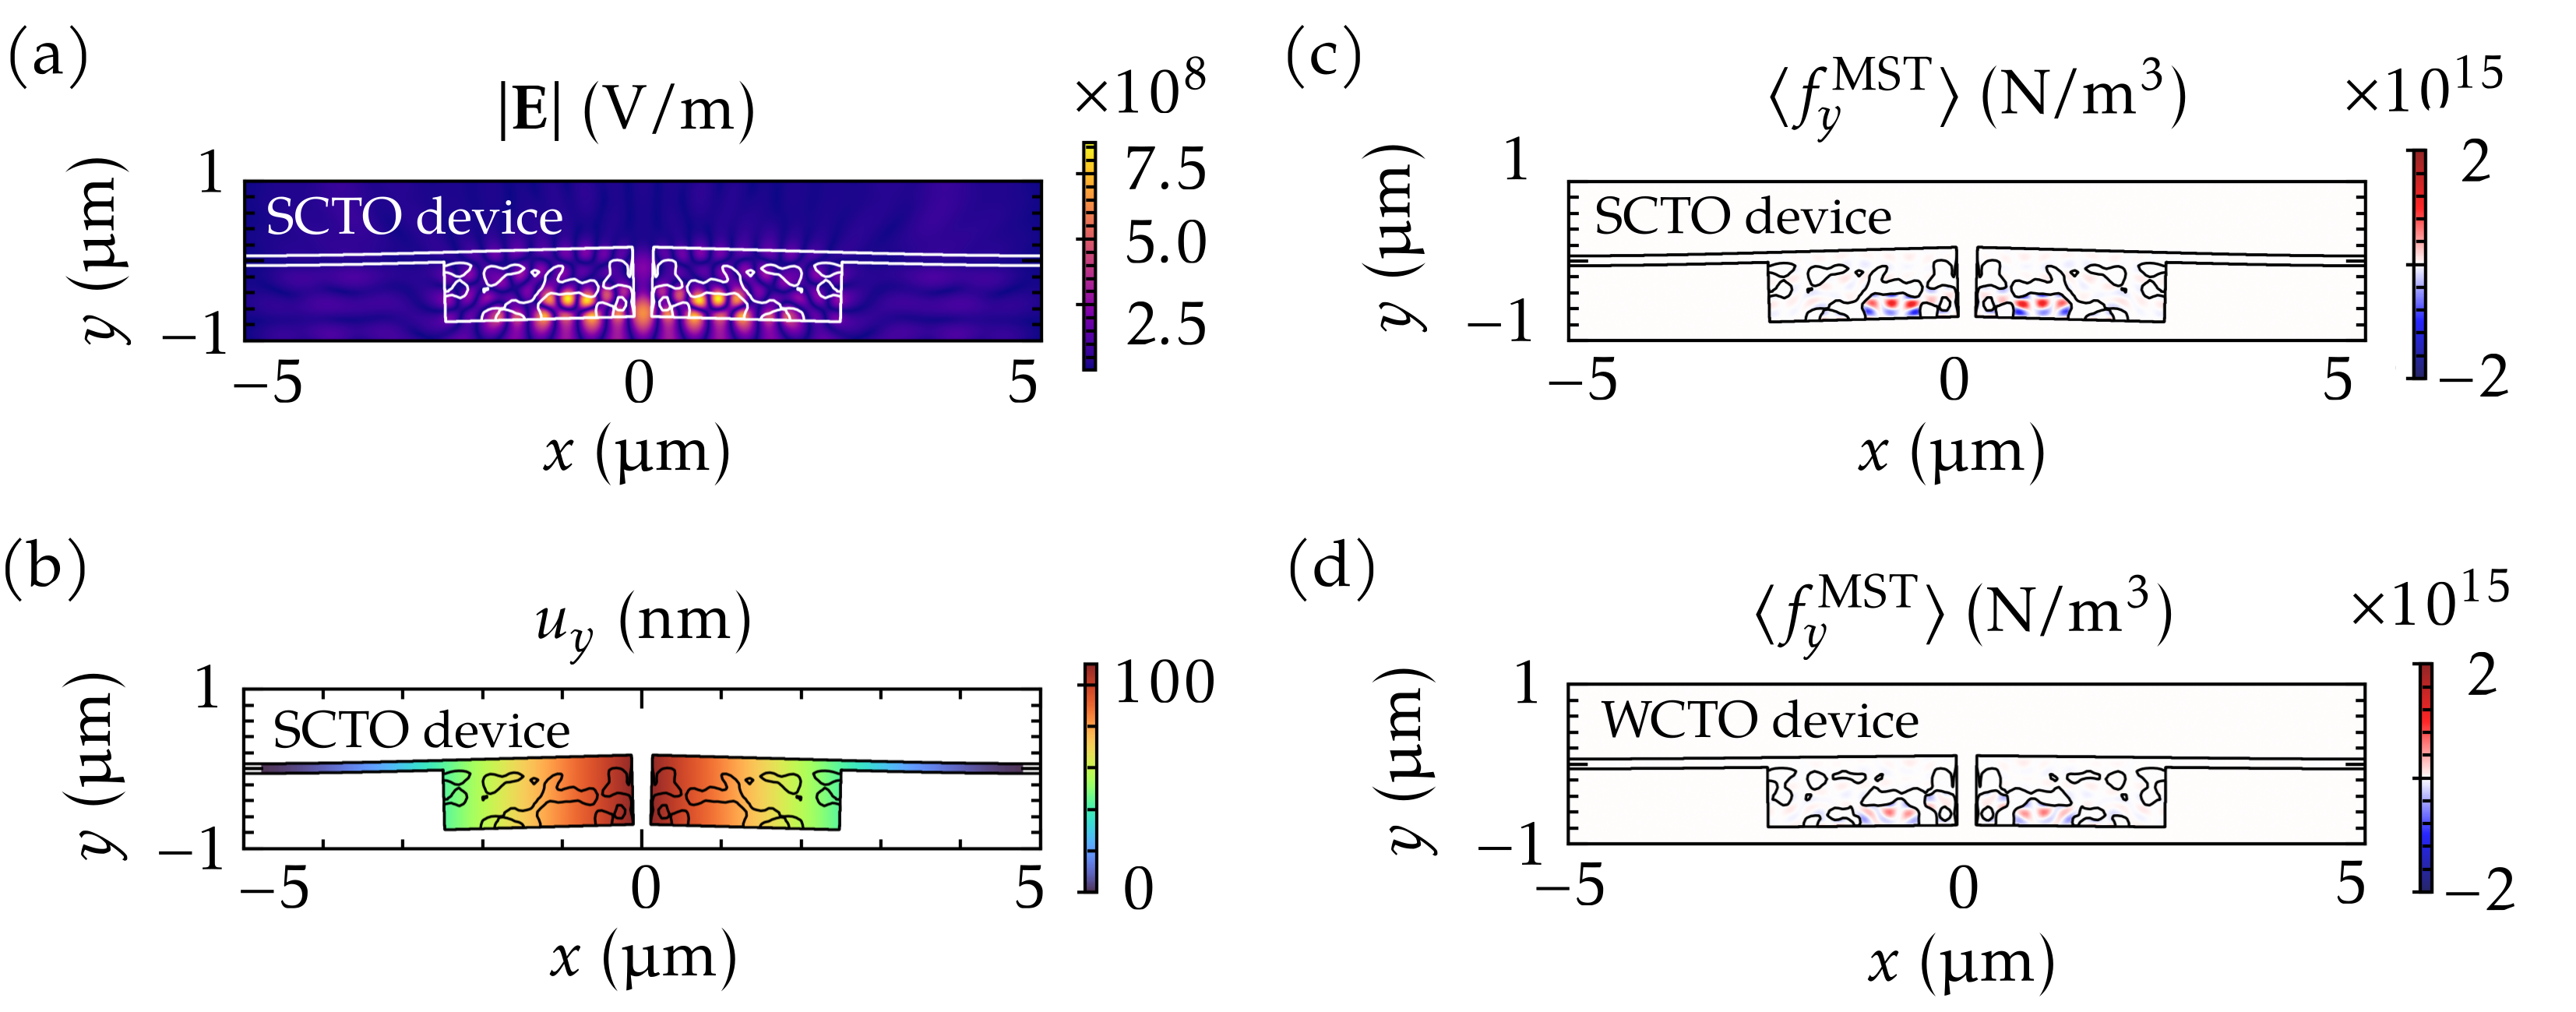
\includegraphics{figures/fields_panels_SC.png}}%%
    \caption{Device evaluation in the deformed material configuration. (a) Electric-field norm ($\vert\mathbf{E}\vert$) for the SCTO device. (b) Vertical displacement ($u_y$) for the SCTO device.
     (c) Vertical ($y$) component of the volumetric force density ($\langle f^\text{MST}_y\rangle$) for the SCTO device. (d) Vertical ($y$) component of
      the volumetric force density ($\langle f^\text{MST}_y\rangle$) for the WCTO device. Adapted from~\cite{ownpub5}.}
    \label{fig:SC}
\end{figure}


Using this formalism, we optimize a membrane-like device with a central hole that spans its full height and splits it along the $x$-axis\footnote{In~\cite{ownpub5}, we also optimize a connected membrane-like device without a central hole.}. We optimize the design based on two models: the strongly 
coupled ($\alpha = 1$, SC) and the weakly coupled ($\alpha = 0$, WC) models. We refer to the optimized devices as SCTO 
(strongly coupled topology-optimized) and WCTO (weakly coupled topology-optimized). Moreover, when evaluating the 
figure of merit, we use the notation $\text{FOM}^a_b$, where the superscript $a$ indicates the model type and the subscript $b$ indicates the device. 
When evaluated with the strongly coupled model, the SCTO device achieves $\text{FOM}^\text{SC}_\text{SCTO}\approx 110$\, nm, while the WCTO achieves only
$\text{FOM}^\text{SC}_\text{WCTO}\approx 43$\,nm, demonstrating a $\approx$3$\times$ improvement when the strong coupling
 is accounted for during optimization. Evaluating the WCTO using the
 weakly coupled model gives $\text{FOM}^\text{WC}_\text{WCTO}\approx$69\,nm, highlighting
 a significant performance drop (a $\approx 0.4 \times$ change in the FOM) due to neglecting the coupling effects in the design process. 
        
        
 Based on the results in \figref{fig:SC}, we see that the SCTO device efficiently reflects
 the incoming plane wave [\figref{fig:SC}(a)], generating a strong optical force distribution
 [\figref{fig:SC}(c)] that leads to significant deformation [\figref{fig:SC}(b)]. 
 The SCTO design outperforms the WCTO design because the devices rotate, causing heterogeneous
 vertical displacements that reduce the ability of the WCTO device to reflect light effectively and weaken the
 optical forces [\figref{fig:SC}(d)]. As a result, the SCTO develops Bragg-mirror-like features
 that are slightly tilted compared to those in the WCTO, improving reflection of the incoming field
 and yielding larger deformations compared to the WCTO device [\figref{fig:SC}(b)].
        

\subsection*{Outlook and future work}
This topology optimization framework for strongly coupled optomechanical systems can be applied to a wide
 range of optomechanical devices and paves the way for future developments. 
 For example, extending the method to include clamping losses and three-dimensional designs
  would improve accuracy for high aspect-ratio membranes~\cite{aspect_ratio}, while including
   photoelastic effects would capture strain-induced refractive index changes~\cite{photoelasticity}.
    The framework also holds promise for cavity optomechanics~\cite{cav_opt} beyond the quasistatic
     regime by replacing the mechanical steady-state model with a frequency-domain solver. 
     Moreover, incorporating models like third-medium regularization~\cite{HuHu0} could enable the design of
      flexible or reconfigurable systems where large deformations and mechanical nonlinearities
       strongly affect optical performance.

       While these advancements are promising, addressing remaining challenges remains critical. Strong plane-wave excitations can induce large displacements and nonlinearities, 
       leading to potential numerical instability. Possible remedies include regularization techniques~\cite{HuHu0}, 
       robust material models, and systematic load ramping. Additionally, further quantifying the trade-offs between
        computational cost and accuracy for WCTO and SCTO designs will help determine when strong coupling is essential
         and when weak coupling is sufficient within acceptable error margins.
